\chapter{Introduction}

    Bla bla intro stuff


\chapter{Performance analysis}

    What is it, problem context, existing solutions in general


\chapter{Project design}

    \section{Freud}

        Brief description, intro to Freud and PIN, what they do and how

    \section{Requirements and analysis}

        Goals, what I needed to implement, refer to the plan and list of tasks, what's the idea

        Develop a simple distributed application based on an RPC library to be used as an initial test environment

        Develop an instrumentation for the client side, server side, and – crucially – the RPC library

        Devise a method to save and retrieve measurement logs from all the remote components

        Design an algorithm to merge the logs from all the systems into a single coherent trace

        Integrate said trace in the existing statistics tool (freud-statistics) to derive the performance annotations

        Identify some third-party non-trivial distributed applications and analyze them with the created tool

        Write the report, prepare the poster and presentation
        
        Have a pizza
        

\chapter{Implementation}
    
    \section{Technologies and tools used}

        Used gRPC \cite{gRPCdocs} as the RPC library, 
        freud-statistics \cite{freud} to analyze the output,
        
        bumped compiler to C++17 for \texttt{filesystem::exists()}

    \section{Issues}

        Made some choices to simplify structure initially, but then had to change it and
        refactor everything

        Problems making sense of the numbers returned by \texttt{freud-statistics} and unable
        to see what was in the binary file to check if I was dumping correctly

        Had to develop some particular encodings since passing from data to text and from text
        to data

        \begin{figure}[H]
            \centering
            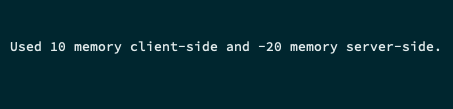
\includegraphics{memUsage.png}
            \caption{A very peculiar memory usage}
            \label{fig:memUsage}
        \end{figure}


\chapter{Evaluation}

    Code validation, analysis of results and practical applications, personal experience

    No coverage/automated tests due to the complexity and erratic nature of the software


\chapter{Conclusions}

    Results wrt objectives, limitations

    Thanks to my advisor, Daniele and everyone that supported me

	\section{Future work and possible developments}

        Re: what the next guy will have to work on next year

        Better handling of the data dumping/efficiency (separate thread)

        Integration with PIN (very hard)

        Support more complex features (re: freud's CLASS type or something)
